\documentclass[ngerman,final,fontsize=12pt,paper=a4,twoside,BCOR=8mm,draft=false]{scrartcl}

\usepackage[T1]{fontenc}
\usepackage{babel}
\usepackage[utf8]{inputenc}
\usepackage[numbers,sort&compress,square]{natbib}
\usepackage[draft=false,final,plainpages=false,pdftex]{hyperref}
\usepackage{graphicx} 

\usepackage[charter,sfscaled]{mathdesign}

\usepackage[spacing=true,tracking=true,kerning=true,babel]{microtype}

\author{GuttenPlag}
\title{Zwischenbericht --- Kollaborative Dokumentation von Plagiaten in der Dissertation „Verfassung und Verfassungsvertrag: Konstitutionelle Entwicklungsstufen in den USA und der EU“ von Karl-Theodor Freiherr zu Guttenberg}

\hypersetup{%
        pdfauthor={GuttenPlag},%
	pdftitle={Zwischenbericht --- Kollaborative Dokumentation von Plagiaten in der Dissertation „Verfassung und Verfassungsvertrag: Konstitutionelle Entwicklungsstufen in den USA und der EU“ von Karl-Theodor Freiherr zu Guttenberg}%
        pdflang={en},%
        pdfduplex={DuplexFlipLongEdge},%
        pdfprintscaling={None}%
}

\begin{document}
\addtokomafont{sectionentry}{\normalfont\bfseries}
\addtokomafont{disposition}{\normalfont\boldmath\bfseries}

\maketitle
\tableofcontents

\section{Einleitung}
Das Guttenplag-Wiki untersucht die veröffentlichte Fassung der Dissertation „Verfassung und Verfassungsvertrag. Konstitutionelle Entwicklungsstufen in den USA und der EU“ des Bundesministers Karl-Theodor zu Guttenberg auf mögliche Plagiatstellen.
Dieser Zwischenbericht dokumentiert erste Ergebnisse unserer Arbeit. Die gefundenen Plagiate erlauben es der akademischen und allgemeinen Öffentlichkeit, sich selbst ein Bild des Falls zu machen.

Ein detaillierter, kontinuierlich erweiterter Bericht der Projektergebnisse findet sich unter http://de.guttenplag.wikia.com/wiki/Guttenberg-2006

Das Wiki und die Beschreibung des Projektziels ist unter http://de.guttenplag.wikia.com/wiki/GuttenPlag\_Wiki einsehbar.

Viele Fragen, die uns im Zusammenhang mit dem Wiki immer wieder gestellt werden, haben wir im Wiki unter http://de.guttenplag.wikia.com/wiki/FAQ (Frequently asked questions, dt. Häufig gestellte Fragen) zusammengestellt und dort beantwortet.

Im Folgenden beschreiben wir zuerst unsere Vorgehensweise und Definitionen. Anschließend dokumentieren wir die vorläufigen Ergebnisse unserer Auswertungen und geben eine vorläufige Bewertung ab.

\section{Vorgehensweise}
Die Analyse der Dissertation fand in mehreren Schritten statt.
\subsection{CrowdSourcing-Phase}
In einem ersten Schritt, der sehr große mediale Aufmerksamkeit erhielt, dokumentierten Hunderte von Benutzern vermutete Plagiate. Wie auch bei Wikipedia war dies anonym möglich. Einordnungen und Quellenangaben wurden in den Kommentaren zu jeder Seite dokumentiert. Diese Suche läuft immer noch. Bis jetzt wurden auf 271 Seiten, über die gesamte Dissertation verteilt, Plagiate gemeldet. Die Liste der gefundenen Seiten findet sich unter http://de.guttenplag.wikia.com/wiki/Plagiate
\subsection{Definition von Plagiats-Kategorien}
Für eine detailliertere Analyse der Fundstellen unterscheiden wir zwischen verschiedenen Arten von Plagiaten. Diese Plagiatskategorien basieren teilweise auf dem Paper \textquotedblleft Strategien und Plagiatsbekämpfung \textquotedblright (Weber-Wulff und Wohnsdorf, erschienen in Information - Wissenschaft \& Praxis, Nr. 2 (März 2006), S. 90-98).
Die von uns verwendeten Kategorien sind:
\begin{itemize}
\item \textbf{Komplettplagiat} 
Komplette Abschnitte der Quelle wurden wörtlich und ohne Zitat übernommen. Dabei haben wir unterschieden, ob die Quelle an einer anderen Stelle im Literaturverzeichnis auftaucht (und damit die Fußnote und Anführungszeichen nur "`vergessen"' wurden) oder ob die Quelle überhaupt nicht erwähnt ist. Beispiele für diese erste Kategorie lassen sich auf Seite 117 (http://de.guttenplag.wikia.com/wiki/Guttenberg-2006/117) und Seite 369 (http://de.guttenplag.wikia.com/wiki/Guttenberg-2006/369)

\item \textbf{Verschleierung} 
Verschleierungen sind Textstellen, die erkennbar von fremden Quellen abstammen, aber umformuliert und weder als Paraphrase noch als Zitat erkennbar gemacht wurden. Gemeint sind Texte, die wegen der Umformulierung nicht mehr einfach als "`Gänsefüßchen/Fußnote vergessen"' abgetan werden können. Diese Neuformulierung dient unter Umständen auch dazu, die Herkunft aus fremder Quelle zu verschleiern. Derlei Plagiate sind beispielsweise auf den Seiten 144 (http://de.guttenplag.wikia.com/wiki/Guttenberg-2006/144), 273, 274 und anderen zu finden.

\item \textbf{Übersetzungsplagiat} 
Ein Übersetzungsplagiat entsteht durch wörtliche Übersetzung aus einem fremdsprachlichen Text. Natürlich lässt hier die Qualität der Übersetzung einen mehr oder weniger großen Interpretationsspielraum, ob tatsächlich ein Plagiat vorliegt oder nicht. Auch ist durch die Übersetzung an sich schon eine mehr oder weniger große Eigenleistung erbracht worden. Nichtsdestotrotz werden fremde Gedankengänge übernommen, ohne dies ersichtlich zu machen. Beispiele für derlei nicht gekennzeichnete Übersetzungen finden sich auf den Seiten 226 (http://de.guttenplag.wikia.com/wiki/Guttenberg-2006/226) bis 229 und Seiten 362 (http://de.guttenplag.wikia.com/wiki/Guttenberg-2006/362) bis 369.

\item \textbf{Bauernopfer} 
In diesem Fall wird zwar eine Fußnote angegeben, diese bezieht sich jedoch auf einen unbedeutenden Teil eines Originaltexts, während größere Abschnitte aus demselben ohne Zitatnachweis übernommen werden und damit den Eindruck einer eigenen Denkleistung erwecken. Beispiele für diese Form von Plagiaten sind auf den Seiten 113 (http://de.guttenplag.wikia.com/wiki/Guttenberg-2006/113), 143, 169 und 338 u.a.

\item \textbf{Verschärftes Bauernopfer} 
In dieser verschärften Variante des Bauernopfers führt die Fußnote den Originaltext mit "`so auch"' an und suggeriert eigenständige Formulierungen, obwohl plagiiert wurde. Beispiele dafür sind auf den Seiten 49 bis 51, 250 und 299.
\item \textbf{Weitere Kategorien} 
Daneben gibt es noch weitere Plagiats-Kategorien und interne Kategorien, z.B. um auf verdächtige Stellen hinzuweisen. Eine komplette Liste der Plagiats-Kategorien finden Sie unter http://de.guttenplag.wikia.com/wiki/PlagiatsKategorien.
\end{itemize}

\subsection{Zur Datenbasis: die Definition und Kategorisierung von "`Fragmenten"'}
Um die von Nutzern des Wiki mitgeteilten Verdachtsfälle bewerten und quantifizieren zu können, wurden die als mögliches Plagiat gemeldeten Seiten in so genannte "`Fragmente"' unterteilt. Als Fragment zählt ein plagiierter Satz, Absatz oder eine Seite der Dissertation, sofern sie
\begin{itemize}
\item sich auf exakt eine Quelle beziehen,
\item genau einer Plagiatskategorie zuzuordnen sind,
\item spätestens am Ende einer Seite enden.
\end{itemize}
Fußnoten wurden immer als eigenständige Fragmente erfasst. Einen Überblick über die bislang erfaßten Fragmente finden Sie hier. 
Für die Erfassung der Fragmente galten die folgenden Richtlinien: 
\begin{itemize}
\item Namensgebung: Der Name des Fragments wird nach folgender Regel gebildet: Fragment\_\$Seite\_\$ZeileVon-\$ZeileBis. (d.h. zwischen \$ZeileVon und \$ZeileBis einen Bindestrich).
\item Seite und Zeilenangaben im Seitennamen beziehen sich auf die Dissertation. Fußnoten (Fn] beginnen immer mit Zeilennummer 101. Alles was Text enthält (außer die Kopfzeile mit der Seitenzahl), wird als Zeile gezählt, auch Überschriften.
\item Umgang mit Seitenumbrüchen: Im Text der Dissertation wird auch ein Satz, der über das Seitenende hinausgeht, stehen gelassen. Der Teil des Satzes, der wegen eines Seitenwechsels am Anfang oder Ende eines Fragments nicht Bestandteil des Fragments ist, ist in eckige Klammern zu setzen. Z.B.: "`[Ich habe] nicht plagiiert"' wenn "`Ich habe"' noch auf der vorherigen Seite steht.
\item Alle Fragmente werden den in ihnen benutzten Quellen zugeordnet. Deren bibliografische Angaben sind jeweils im Fragment verzeichnet. Die Zusammenführung dieser Daten muss in der nächsten Arbeitsphase noch vervollständigt werden.
\end{itemize}

\subsection{Verifizierung und Archivierung}
Parallel zur Fragment-Kategorisierung werden diese Fragmente auf http://de.guttenplag.wikia.com/wiki/Guttenberg-2006 archiviert. Neben Verweisen zu allen Einzelseiten, die jeweils alle auf einer Seite der Dissertation gefundenen Plagiate zusammenfassen, entsteht hier eine Kurzstatistik über den Umfang der Plagiation sowie den Arbeitsfortschritt. Momentan sind 139 Seiten auf diese Weise verfügbar. 
Als zukünftiger Arbeitsschritt ist geplant, die hier zusammengefassten Fragmente mehrfach zu sichten und auf Fehler/Plausibilität zu prüfen. Das Ergebnis dieser Sichtung steht dann als geschütztes Archiv der Bemühungen dauerhaft zur Verfügung.

\section{Ergebnisse}
Im Folgenden dokumentieren wir einige vorläufige Ergebnisse. Besonderes Augenmerk gilt den bereits analysierten Fundstellen.

\subsection{Herausragende Fundstellen}
Aus der Vielzahl der Fundstellen ragen einige heraus, die sich durch ihre Position in der Dissertation, durch ihre Art oder durch ihre ungewöhnliche Quelle auszeichnen. Einige Beispiele sind hier aufgeführt, die komplette Liste der herausragenden Fundstellen ist unter http://de.guttenplag.wikia.com/wiki/Herausragende\_Fundstellen zu finden. 

Schon die Einleitung beginnt mit einem Plagiat: "`E pluribus unum"' mitsamt nachfolgendem Absatz ist ein aus einem FAZ-Artikel von Barbara Zehnpfennig übernommenes Komplettplagiat (http://de.guttenplag.wikia.com/wiki/Guttenberg-2006/015). 

Die dazugehörige Fußnote (hier: http://de.guttenplag.wikia.com/wiki/Fragment\_015\_108-118) ist gleich wieder ein Plagiat, diesmal aus der "`Fischer Länderkunde Nordamerika"', einer für juristische Dissertationen ungewöhnlichen Quelle, entlehnt. 

Mehrere Plagiate tauchen gleich mehrfach im Text auf. Sowohl auf Seite 196 als auch auf Seite 264 der Arbeit wird der gleiche Text von Gebhardt (hier: http://de.guttenplag.wikia.com/wiki/Kategorie:Gebhardt\_1987) verwendet; Wassers (hier: http://de.guttenplag.wikia.com/wiki/Kategorie:Wasser\_1997) Ausführungen zur Judiziokratie finden wörtliche Verwendung auf den Seiten 276 und 288. 

Übersetzungsplagiate finden sich zahlreich, herausragend davon ist ein Abschnitt über mehr als sechs Seiten (362-363, 363-364 und weitere), der Satz für Satz aus einem Artikel in "`Foreign Policy"' (hier zu finden: http://de.guttenplag.wikia.com/wiki/Kategorie:Rakove\_2003) übersetzt wurde.

\subsection{Unerwähnte Quellen}

Zahlreiche Quellen werden abgeschrieben, ohne sie in Fußnoten oder im Literaturverzeichnis aufzuführen. Insbesondere betrifft dies:
\begin{itemize}

\item die Erstsemester-Hausarbeit von Daniel Pentzlin (http://de.guttenplag.wikia.com/wiki/Kategorie:ZBhausarbeitUNBEKANNT\_2003)
\item eine Masterarbeit von Dörte Ratzmann (2003) (http://de.guttenplag.wikia.com/wiki/Kategorie:Ratzmann\_2003)
\item eine Studienarbeit von Diana Bauer (2002) (http://de.guttenplag.wikia.com/wiki/Kategorie:Bauer\_2002)
\item einen US-Botschaftsbericht (http://de.guttenplag.wikia.com/wiki/Kategorie:U.S.\_Diplomatic\_Mission\_to\_Germany\_2004)
\item eine historische Studie von Udo Sautter (1976) (http://de.guttenplag.wikia.com/wiki/Kategorie:Sautter\_1976)
\item einen Zeitungsartikel von Oliver Burgard (DIE ZEIT) (http://de.guttenplag.wikia.com/wiki/Kategorie:Burgard\_2000)

\item und andere Schriften, zum Beispiel von der Verwaltung des Deutschen Bundestags (2006) (http://de.guttenplag.wikia.com/wiki/Kategorie:Bundestag\_2006), Hans-Gerd Pieper (1998) (http://de.guttenplag.wikia.com/wiki/Kategorie:Pieper\_1998), Brigitte Marcher (2002) (http://de.guttenplag.wikia.com/wiki/Kategorie:Marcher\_2002), Nadja Janssen (2005) (http://de.guttenplag.wikia.com/wiki/Kategorie:Janssen\_2005), Hagen Schulze (1999) (http://de.guttenplag.wikia.com/wiki/Kategorie:Schulze\_1999), Hartmut Wasser (1997) (http://de.guttenplag.wikia.com/wiki/Kategorie:Wasser\_1997), Stefan Schieren (2002) (http://de.guttenplag.wikia.com/wiki/Kategorie:Schieren\_2002), Dr. Andreas Schwab (2001) (http://de.guttenplag.wikia.com/wiki/Kategorie:Schwab\_2001), und Maria Duftner (2001) (http://de.guttenplag.wikia.com/wiki/Kategorie:Duftner\_2001).
\end{itemize}
Andere Quellen werden zwar anderswo in Fussnoten erwähnt, stehen aber nicht im Literaturverzeichnis der Arbeit, obwohl auch von dort abgeschrieben wurde, z. B. Claus Giering (http://de.guttenplag.wikia.com/wiki/Kategorie:Giering), Georg Kreis (2003) (http://de.guttenplag.wikia.com/wiki/Kategorie:Kreis\_2003), Anne Peters (2004) (http://de.guttenplag.wikia.com/wiki/Kategorie:Peters\_2004), und Wolfgang Reinhard (1999) (http://de.guttenplag.wikia.com/wiki/Kategorie:Reinhard)

\subsection{Unverifizierte Fundstellen}

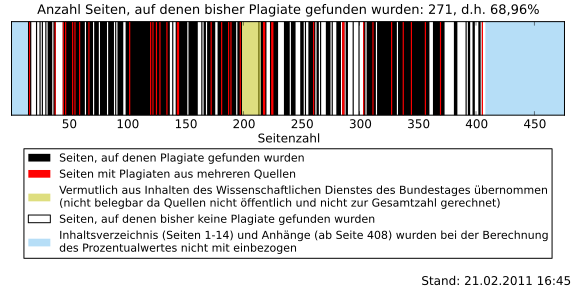
\includegraphics[scale=0.6]{Barcode-Zwischenbericht}

\subsection{Analysierte Fundstellen}

Es wurden inzwischen über 160 der insgesamt 271 als Plagiat gemeldeten Seiten analysiert und in oben genannten "`Fragmenten"' dokumentiert. Die 302 Fragmente, die im Allgemeinen jeweils einer plagiierten Stelle entsprechen, wurden einmal auf Plausibilität überprüft, aber noch nicht doppelt verifiziert.
Eine statistische Auswertung (Script) nur der bereits analysierten Fragmente zeigt:

\begin{itemize}
\item 1115 Zeilen (~27 Seiten reiner Text) sind Komplettplagiate aus anderen Quellen.
\item Weitere 1437 Zeilen (35 Seiten reiner Text) sind verschleierte Plagiate, d.h. keinesfalls durch vergessene Anführungszeichen entstanden.
\item Hinzu kommen \begin{itemize}
      \item 410 Zeilen Übersetzungsplagiate,
      \item 121 Zeilen die als Bauernopfer klassifiziert wurden und
      \item 438 Zeilen als verschärfte Bauernopfer. \end{itemize}
\item Bei 8 Fragmenten wollen wir noch keine Aussage treffen.
\end{itemize}
Dies bedeutet, dass bis jetzt 3521 von 16325 Zeilen, das sind 21,5\% der Doktorarbeit (jeweils inkl. Fußnoten) als Plagiate identifiziert wurden.

Die einzelnen Fragmente können hier: http://de.guttenplag.wikia.com/wiki/Spezial:Präfixindex/Fragment oder über http://daten.dieweltistgarnichtso.net/src/guttenviz/ betrachtet werden. Eine Gegenüberstellung von gescannter Dissertation und Originalquellen findet sich unter http://gut.greasingwheels.org/. Durch die automatisierte Annotierung ist die Darstellung in manchen Fällen fehlerhaft.

\section{Bewertung}
Aus den in diesem Zwischenbericht dokumentierten Plagiaten lassen sich folgende Schlussfolgerungen ziehen:
\begin{itemize}
\item In der Dissertation wurden in erheblichem Ausmaß fremde Quellen verwendet, die nicht als Zitat gekennzeichnet wurden. Dies ist eine eklatante Verletzung der wissenschaftlichen Arbeitsweise.
\item Die zahlreichen textuellen Anpassungen der Plagiate, die Tatsache, dass die Plagiate über die ganze Dissertation hinweg zu finden sind, und die Tatsache, dass selbst die Einleitung kopiert wurde, lassen darauf schließen, dass diese Plagiate kein Versehen waren, sondern bewusst getätigt wurden.
\end{itemize}
\section{Weiteres Vorgehen}
Dieser Bericht stellt, wie in der Einleitung schon erwähnt, eine Zwischenbilanz dar. Die Dynamik dieser Affäre war nicht vorhersehbar und hat auch uns überrascht. Der Umfang der vermuteten Plagiate ist in den letzten Tagen geradezu explodiert. Aufgrund dieser wachsenden Datenmasse und der damit einhergehenden kurzen/begrenzten Prüfungszeit sind die hier dokumentierten Textstellen immer noch mit Unsicherheit behaftet. Unser Ziel ist eine detaillierte Analyse dieser vermuteten Plagiate. Die Arbeit am GuttenPlag-Wiki wird fortgesetzt und wir freuen uns über jede helfende Hand. Auch möchten wir uns schon jetzt bei den vielen Menschen bedanken, die dieses Projekt so erfolgreich gemacht haben. Sobald wir alle gemeldeten Fundstellen analysiert haben, werden wir unsere Erkenntnisse ausführlich in einem Abschlussbericht dokumentieren. Hierfür können wir momentan keinen konkreten Termin nennen. 

Die Entscheidung über den Entzug des Doktortitels des Freiherrn zu Guttenberg liegt bei der Rechts- und Wirtschaftswissenschaftlichen Fakultät der Universität Bayreuth.

\section{Weiterführende Links}
http://de.guttenplag.wikia.com/wiki/Guttenberg-2006 
http://de.guttenplag.wikia.com/wiki/Chronologie
\end{document}
